\section{Аналитическая часть}

\subsection{Расстояние Левенштейна}

Расстояние Левенштейна --- метрика, определяющая понятие расстояния между двумя последовательностями символов, как минимального количества редакторских операций вставки ($I$, от англ. insert), замены ($R$, от англ. replace) и удаления ($D$, от англ. delete), необходимых для преобразования одной строки в другую \cite{lev}.
Для каждой операции должна быть определена её стоимость.
Введём обозначения для стоимостей.
Пусть:
\begin{enumerate}
    \item $w(a, b)$ --- цена замены символа $a$ на $b$;
    \item $w(\lambda, b)$ --- цена вставки символа $b$;
    \item $w(a, \lambda)$ --- цена удаления символа $a$.
\end{enumerate}

Определим стоимости операций:
\begin{equation}
    w(a, b) = \begin{cases}
        1,\ \text{если}\ a \neq b; \\
        0,\ \text{иначе}.
    \end{cases}
    \label{eq:w}
\end{equation}

Отсутствие операций в случае совпадения символов будем обозначать за $M$ (от англ. match).

Введём в рассмотрение функцию $D(S_1[1 .. i], S_2[1 .. j])$, значнием которой является редакционное расстояние между подстроками $S_1[1 .. i]$ и $S_2[1 .. j]$, где $S_1[1 .. i]$ --- подстрока $S_1$ длины $i$. Так, если $S_1 = \text{\texttt{''скат''}}$, то $S_1[1 .. 0] = \lambda$, $S_1[1 .. 1] = \text{\texttt{''с''}}$, $S_1[1 .. 2] = \text{\texttt{''ск''}}$.
Расстояние Левенштейна между строками $S_1$ и $S_2$ длин $L_1$ и $L_2$ соответственно вычисляется по рекуррентной формуле:
\begin{multline}
    D(S_1[1 .. i], S_2[1 .. j]) = \\
    = \begin{cases}
        \begin{aligned}
            &\mathrm{max}(i,\ j), &i \cdot j = 0; \\
            &\mathrm{min} \begin{cases}
                D(S_1[1 .. i], S_2[1 .. j - 1]) + 1, \\
                D(S_1[1 .. i - 1], S_2[1 .. j]) + 1, \\
                D(S_1[1 .. i - 1], S_2[1 .. j - 1]) + w(S_1[i], S_2[j]),
            \end{cases} &i \cdot j \neq 0,
        \end{aligned}
    \end{cases}
    \label{eq:lev}
\end{multline}

где $i = L_1$, $j = L_2$.
% где $i = \overline{0;L_1}$, $j = \overline{0;L_2}$.

\subsubsection{Итерационный алгоритм нахождения расстояния Левенштейна}

Рекурсивная реализация алгоритма поиска расстояния Левенштейна малоэффективна по времени при больших $L_1$ и $L_2$, так как производится много повторных, лишних вычислений.
Реализацию можно оптимизировать с помощью динамического программирования.
Например, ввести матрицу размерности $(L_1 + 1) \times (L_2 + 1)$ и заполнять её промежуточными значениями $D(S_1[1 .. i], S_2[1 .. j])$, используя их затем по ходу вычислений.
Значения в ячейках $[i][j]$ ($i$-я строка, $j$-й столбец) матрицы равны значениям $D(S_1[1 .. i], S_2[1 .. j])$ соответственно.
Можно заметить, что всю матрицу для вычислений хранить не обязательно --- двух строк будет достаточно.

\subsection{Расстояние Дамерау --- Левенштейна}

Расстояние Дамерау --- Левенштейна --- метрика, которая определяет расстояние между двумя последовательностями символов, как и расстояние Левенштейна, но к исходному набору редакторских операций добавляется ещё одна --- транспозиция (T, от англ. transposition).
Операция транспозиции меняет местами соседние буквы в строке.
Обозначим её стоимость: $w(ab, ba) = 1$.

Расстояние Дамерау --- Левенштейна $\mathcal{D}(S_1, S_2)$ между строками $S_1$ и $S_2$ длин $L_1$ и $L_2$ соответственно может быть вычислено по рекуррентной формуле:
\begin{multline}
    \mathcal{D}(S_1[1 .. i], S_2[1 .. j]) = \\
    = \begin{cases}
        \begin{aligned}
            &\mathrm{max}(i,\ j), &\text{если}\ i \cdot j = 0; \\
            &\mathrm{min} \begin{cases}
                \mathcal{D}(S_1[1 .. i], S_2[1 .. j - 1]) + 1, \\
                \mathcal{D}(S_1[1 .. i - 1], S_2[1 .. j]) + 1, \\
                \mathcal{D}(S_1[1 .. i - 1], S_2[1 .. j - 1]) + w(S_1[i], S_2[j]), \\
                \mathcal{D}(S_1[1 .. i - 2], S_2[1 .. j - 2]) + 1,
                \end{cases} &\parbox{3.5cm}{
                    \raggedleft если $i > 1,\ j > 1$,
                    $S_1[i] = S_2[j - 1]$,
                    $S_1[i - 1] = S_2[j]$;
                } \\ % XXX: how to do auto width?
            &\mathrm{min} \begin{cases}
                \mathcal{D}(S_1[1 .. i], S_2[1 .. j - 1]) + 1, \\
                \mathcal{D}(S_1[1 .. i - 1], S_2[1 .. j]) + 1, \\
                \mathcal{D}(S_1[1 .. i - 1], S_2[1 .. j - 1]) + w(S_1[i], S_2[j]),
                \end{cases} &\text{иначе},
        \end{aligned}
    \end{cases}
    \label{eq:damlev}
\end{multline}

где $i = L_1$, $j = L_2$.

\subsubsection{Рекурсивный алгоритм нахождения расстояния Дамерау --- Левенштейна}

Рекурсивный алгоритм нахождения расстояния Дамерау --- Левенштейна реализует рекуррентную формулу (\ref{eq:damlev}). Таким образом, верно следующее:
\begin{enumerate}
    \item $\mathcal{D}(\lambda, \lambda) = 0$, --- для преобразования пустой строки в пустую строку требуется $0$ операций вставки, замены, удаления и транспозиции;
    \item $\mathcal{D}(S_1, \lambda) = |S_1|$ (длина $S_1$), --- для преобразования строки $S_1$ в пустую строку требуется $|S_1|$ операций (удаления);
    \item $\mathcal{D}(\lambda, S_2) = |S_2|$, --- для преобразования пустой строки в строку $S_2$ требуется $|S_2|$ операций (вставки);
    \item $\mathcal{D}(c_1, c_2) = \begin{cases}
            \begin{aligned}
                1,\ &c_1 \neq c_2; \\
                0,\ &c_1 = c_2,
            \end{aligned}
    \end{cases} $ --- для преобразования одного символа в другой требуется $1$ операция (замены), если символы отличаются, и $0$ операций, если символы совпадают;
    \item Для преобразования одной пары символов в другую: \\
        $\mathcal{D}(c_1c_2, c_3c_4) = \begin{cases}
            \begin{aligned}
                0,\ &c_1 = c_3,\ c_2 = c_4;\ //\ MM \\
                1,\ &c_1 = c_3,\ c_2 \neq c_4;\ //\ MR \\
                1,\ &c_1 \neq c_3,\ c_2 = c_4;\ //\ RM \\
                1,\ &c_1 = c_4,\ c_2 = c_3;\ //\ T \\
                2,\ &\text{иначе};\ //\ RR
            \end{aligned}
        \end{cases} $
    % \item Для преобразования строки $S_1$, $|S_1| \geq 2$ в строку $S_2$, $|S_2| \geq 2$: $$
    \item Пусть $S_1 = S_1'c_2 = S_1''c_1c_2$, $S_2 = S_2'c_4 = S_2''c_3c_4$, где $S_1'$ и $S_2'$ --- строки $S_1$ и $S_2$ без последних символов, $S_1''$ и $S_2''$ --- строки $S_1$ и $S_2$ без двух последних символов, а $c_1c_2$ и $c_3c_4$ --- пары их последних символов соответственно. $$
    \mathcal{D}(S_1, S_2) = \mathrm{min} \begin{cases}
        % \begin{aligned}
        % \mathcal{D}(S_1''c_1c_2, S_2''c_3) + 1, \\
        % \mathcal{D}(S_1''c_1, S_2''c_3c_4) + 1, \\
        % \mathcal{D}(S_1''c_1, S_2''c_3) + w(c_2, c_4), \\
        % \mathcal{D}(S_1'', S_2''),\ &\text{если $c_2 = c_3,\ c_1 = c_4$}.
        \mathcal{D}(S_1'c_2, S_2') + 1, \\
        \mathcal{D}(S_1', S_2'c_4) + 1, \\
        \mathcal{D}(S_1', S_2') + w(c_2, c_4), \\
        \mathcal{D}(S_1'', S_2'') + 1,\ &\text{если $c_2 = c_3,\ c_1 = c_4$}.
        % \end{aligned}
    \end{cases}
        $$
\end{enumerate}

Можно заметить, что $\mathcal{D}(S_1, S_2)$ вычисляется как минимальная длина последовательности редакторских операций, которыми можно преобразовать строку $S_1$ в $S_2'$ плюс цена вставки последнего символа из $S_2$, строку $S_1'$ в $S_2$ плюс цена удаления последнего символа из $S_1$, строку $S_1'$ в $S_2'$ плюс цена замены последних символов строк $S_1$ и $S_2$, строку $S_1''$ в $S_2''$ плюс цена транспозиции двух последних символов строк, если она возможна.
Для любых подстрок $\mathcal{S}_1$ и $\mathcal{S}_2$ строк $S_1$ и $S_2$, $\mathcal{D}(\mathcal{S}_1, \mathcal{S}_2)$ вычисляет минимальное количество редакторских операций.
Следовательно, $\mathcal{D}(S_1, S_2)$ действительно считает расстояние Дамерау --- Левенштейна для произвольных строк строк $S_1$ и $S_2$.

\subsubsection{Рекурсивный с кешированием алгоритм нахождения расстояния Дамерау --- Левенштейна}

Рекурсивный алгоритм нахождения расстояния Дамерау --- Левенштейна прост, но его реализация на ЭВМ без дополнительных оптимизаций нерациональна, так как по нескольку раз считаются значения, которые уже были вычислены, а вычисление их может оказаться достаточно трудоёмким.

Идея возможной оптимизации состоит в следующем: хранить получаемые по ходу выполнения алгоритма значения в матрице, а перед вычислением очередного --- проверять, было ли оно посчитано ранее (заполнена ли соответствующая ячейка матрицы), и, если да, --- брать его оттуда, не прибегая к повторным вычислениям.

\subsubsection{Итерационный алгоритм нахождения расстояния Дамерау --- Левенштейна}

Как алгоритм поиска расстояния Левенштейна, так и алгоритм поиска расстояния Дамерау --- Левенштейна можно реализовать нерекурсивно с помощью динамического программирования, используя матрицу расстояний.

Процесс вычисления значения ячейки матрицы показан на рисунке \ref{fig:dlmat}.

\begin{figure}[H]
    \begin{center}
        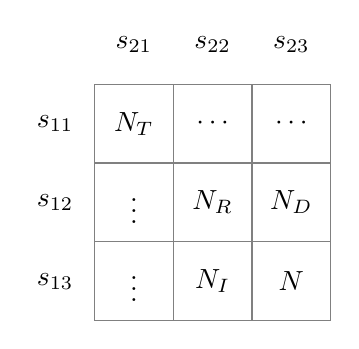
\begin{tikzpicture}
            \draw[step=1.0cm,color=gray] (-1,-1) grid (2,2);
            \node at (-1.50,+1.50) {$s_{11}$};
            \node at (-1.50,+0.50) {$s_{12}$};
            \node at (-1.50,-0.50) {$s_{13}$};
            \node at (-0.50,+2.50) {$s_{21}$};
            \node at (+0.50,+2.50) {$s_{22}$};
            \node at (+1.50,+2.50) {$s_{23}$};
            \node at (-0.50,+1.50) {$N_T$};
            \node at (+0.50,+1.50) {$\cdots$};
            \node at (+1.50,+1.50) {$\cdots$};
            \node at (-0.50,+0.50) {$\vdots$};
            \node at (-0.50,-0.50) {$\vdots$};
            \node at (+0.50,+0.50) {$N_R$};
            \node at (+1.50,+0.50) {$N_D$};
            \node at (+0.50,-0.50) {$N_I$};
            \node at (+1.50,-0.50) {$\boldsymbol{N}$};
        \end{tikzpicture}

        \( \boldsymbol{N} =
        % \mathcal{D}(S_1, S_2) = 
        \mathrm{min} \begin{cases}
    N_I + 1, \\
    N_D + 1, \\
    N_R + w(s_{13}, s_{23}), \\
            \begin{cases}
                N_T + 1,\ &\text{если $s_{13} = s_{22},\ s_{12} = s_{23}$ и $s_{11}$, $s_{21}$ существуют}, \\
                \infty,\ &\text{иначе}.
            \end{cases}
\end{cases} \)
    \end{center}
    \caption{Вычисление расстояния Дамерау --- Левенштейна с использованием матрицы}
    \label{fig:dlmat}
\end{figure}

Таким образом, для нахождения расстояния Дамерау --- Левенштейна хранить всю матрицу не обязательно --- трёх строк будет достаточно.
Заполнив последнее значение очередной строки, можно выполнить <<циклическую прокрутку>> строк матрицы вверх, после чего изменить значение первой ячейки последней теперь строки матрицы на значение первой ячейки предпоследней строки матрицы плюс $1$, а затем продолжить заполнение матрицы по алгоритму, представленному на рисунке выше, перезаписывая значения ячеек.
